\documentclass[a4paper,justified,final,twoside,nobib]{tufte-book}

\hypersetup{colorlinks}% uncomment this line if you prefer colored hyperlinks (e.g., for onscreen viewing)

\usepackage{mathtools} %added mathtools for piecewise functions

%%
% Book metadata
\title{A\\Machine Learning\\Handbook\thanks{Thanks to Edward R.~Tufte for his inspiration.}}
\author[]{}
\publisher{Publisher of This Book}

%%
% If they're installed, use Bergamo and Chantilly from www.fontsite.com.
% They're clones of Bembo and Gill Sans, respectively.
%\IfFileExists{bergamo.sty}{\usepackage[osf]{bergamo}}{}% Bembo
%\IfFileExists{chantill.sty}{\usepackage{chantill}}{}% Gill Sans

\usepackage{microtype}

%%
% Just some sample text
\usepackage{lipsum}
\usepackage{soul}
%%
% For nicely typeset tabular material
\usepackage{booktabs}
\usepackage{pdfpages}

%%
% For graphics / images
\usepackage{graphicx}
\setkeys{Gin}{width=\linewidth,totalheight=\textheight,keepaspectratio}
\graphicspath{{graphics/}}

% The fancyvrb package lets us customize the formatting of verbatim
% environments.  We use a slightly smaller font.
\usepackage{fancyvrb}
\fvset{fontsize=\normalsize}

%%
% Prints argument within hanging parentheses (i.e., parentheses that take
% up no horizontal space).  Useful in tabular environments.
\newcommand{\hangp}[1]{\makebox[0pt][r]{(}#1\makebox[0pt][l]{)}}

%%
% Prints an asterisk that takes up no horizontal space.
% Useful in tabular environments.
\newcommand{\hangstar}{\makebox[0pt][l]{*}}

%%
% Prints a trailing space in a smart way.
\usepackage{xspace}

%%
% Some shortcuts for Tufte's book titles.  The lowercase commands will
% produce the initials of the book title in italics.  The all-caps commands
% will print out the full title of the book in italics.
\newcommand{\vdqi}{\textit{VDQI}\xspace}
\newcommand{\ei}{\textit{EI}\xspace}
\newcommand{\ve}{\textit{VE}\xspace}
\newcommand{\be}{\textit{BE}\xspace}
\newcommand{\VDQI}{\textit{The Visual Display of Quantitative Information}\xspace}
\newcommand{\EI}{\textit{Envisioning Information}\xspace}
\newcommand{\VE}{\textit{Visual Explanations}\xspace}
\newcommand{\BE}{\textit{Beautiful Evidence}\xspace}
\newcommand{\ics}{\smallcaps{ICS5110 Applied Machine Learning\xspace}}

\newcommand{\TL}{Tufte-\LaTeX\xspace}

% Prints the month name (e.g., January) and the year (e.g., 2008)
\newcommand{\monthyear}{%
  \ifcase\month\or January\or February\or March\or April\or May\or June\or
  July\or August\or September\or October\or November\or
  December\fi\space\number\year
}

% Prints an epigraph and speaker in sans serif, all-caps type.
\newcommand{\openepigraph}[2]{%
  %\sffamily\fontsize{14}{16}\selectfont
  \begin{fullwidth}
  \sffamily\large
  \begin{doublespace}
  \noindent\allcaps{#1}\\% epigraph
  \noindent\allcaps{#2}% author
  \end{doublespace}
  \end{fullwidth}
}

% Inserts a blank page
\newcommand{\blankpage}{\newpage\hbox{}\thispagestyle{empty}\newpage}

\usepackage{units}

% Typesets the font size, leading, and measure in the form of 10/12x26 pc.
\newcommand{\measure}[3]{#1/#2$\times$\unit[#3]{pc}}

% Macros for typesetting the documentation
\newcommand{\hlred}[1]{\textcolor{Maroon}{#1}}% prints in red
\newcommand{\hangleft}[1]{\makebox[0pt][r]{#1}}
\newcommand{\hairsp}{\hspace{1pt}}% hair space
\newcommand{\hquad}{\hskip0.5em\relax}% half quad space
\newcommand{\TODO}{\textcolor{red}{\bf TODO!}\xspace}
\newcommand{\ie}{\textit{i.\hairsp{}e.}\xspace}
\newcommand{\eg}{\textit{e.\hairsp{}g.}\xspace}
\newcommand{\na}{\quad--}% used in tables for N/A cells
\providecommand{\XeLaTeX}{X\lower.5ex\hbox{\kern-0.15em\reflectbox{E}}\kern-0.1em\LaTeX}
\newcommand{\tXeLaTeX}{\XeLaTeX\index{XeLaTeX@\protect\XeLaTeX}}
% \index{\texttt{\textbackslash xyz}@\hangleft{\texttt{\textbackslash}}\texttt{xyz}}
\newcommand{\tuftebs}{\symbol{'134}}% a backslash in tt type in OT1/T1
\newcommand{\doccmdnoindex}[2][]{\texttt{\tuftebs#2}}% command name -- adds backslash automatically (and doesn't add cmd to the index)
\newcommand{\doccmddef}[2][]{%
  \hlred{\texttt{\tuftebs#2}}\label{cmd:#2}%
  \ifthenelse{\isempty{#1}}%
    {% add the command to the index
      \index{#2 command@\protect\hangleft{\texttt{\tuftebs}}\texttt{#2}}% command name
    }%
    {% add the command and package to the index
      \index{#2 command@\protect\hangleft{\texttt{\tuftebs}}\texttt{#2} (\texttt{#1} package)}% command name
      \index{#1 package@\texttt{#1} package}\index{packages!#1@\texttt{#1}}% package name
    }%
}% command name -- adds backslash automatically
\newcommand{\doccmd}[2][]{%
  \texttt{\tuftebs#2}%
  \ifthenelse{\isempty{#1}}%
    {% add the command to the index
      \index{#2 command@\protect\hangleft{\texttt{\tuftebs}}\texttt{#2}}% command name
    }%
    {% add the command and package to the index
      \index{#2 command@\protect\hangleft{\texttt{\tuftebs}}\texttt{#2} (\texttt{#1} package)}% command name
      \index{#1 package@\texttt{#1} package}\index{packages!#1@\texttt{#1}}% package name
    }%
}% command name -- adds backslash automatically
\newcommand{\docopt}[1]{\ensuremath{\langle}\textrm{\textit{#1}}\ensuremath{\rangle}}% optional command argument
\newcommand{\docarg}[1]{\textrm{\textit{#1}}}% (required) command argument
\newenvironment{docspec}{\begin{quotation}\ttfamily\parskip0pt\parindent0pt\ignorespaces}{\end{quotation}}% command specification environment
\newcommand{\docenv}[1]{\texttt{#1}\index{#1 environment@\texttt{#1} environment}\index{environments!#1@\texttt{#1}}}% environment name
\newcommand{\docenvdef}[1]{\hlred{\texttt{#1}}\label{env:#1}\index{#1 environment@\texttt{#1} environment}\index{environments!#1@\texttt{#1}}}% environment name
\newcommand{\docpkg}[1]{\texttt{#1}\index{#1 package@\texttt{#1} package}\index{packages!#1@\texttt{#1}}}% package name
\newcommand{\doccls}[1]{\texttt{#1}}% document class name
\newcommand{\docclsopt}[1]{\texttt{#1}\index{#1 class option@\texttt{#1} class option}\index{class options!#1@\texttt{#1}}}% document class option name
\newcommand{\docclsoptdef}[1]{\hlred{\texttt{#1}}\label{clsopt:#1}\index{#1 class option@\texttt{#1} class option}\index{class options!#1@\texttt{#1}}}% document class option name defined
\newcommand{\docmsg}[2]{\bigskip\begin{fullwidth}\noindent\ttfamily#1\end{fullwidth}\medskip\par\noindent#2}
\newcommand{\docfilehook}[2]{\texttt{#1}\index{file hooks!#2}\index{#1@\texttt{#1}}}
\newcommand{\doccounter}[1]{\texttt{#1}\index{#1 counter@\texttt{#1} counter}}

% Generates the index
\usepackage{makeidx}
\makeindex

\usepackage{tikz}

\begin{document}
	\begingroup
	\thispagestyle{empty}
	\begin{tikzpicture}[remember picture,overlay]
	\node[inner sep=0pt] (background) at (current page.center) {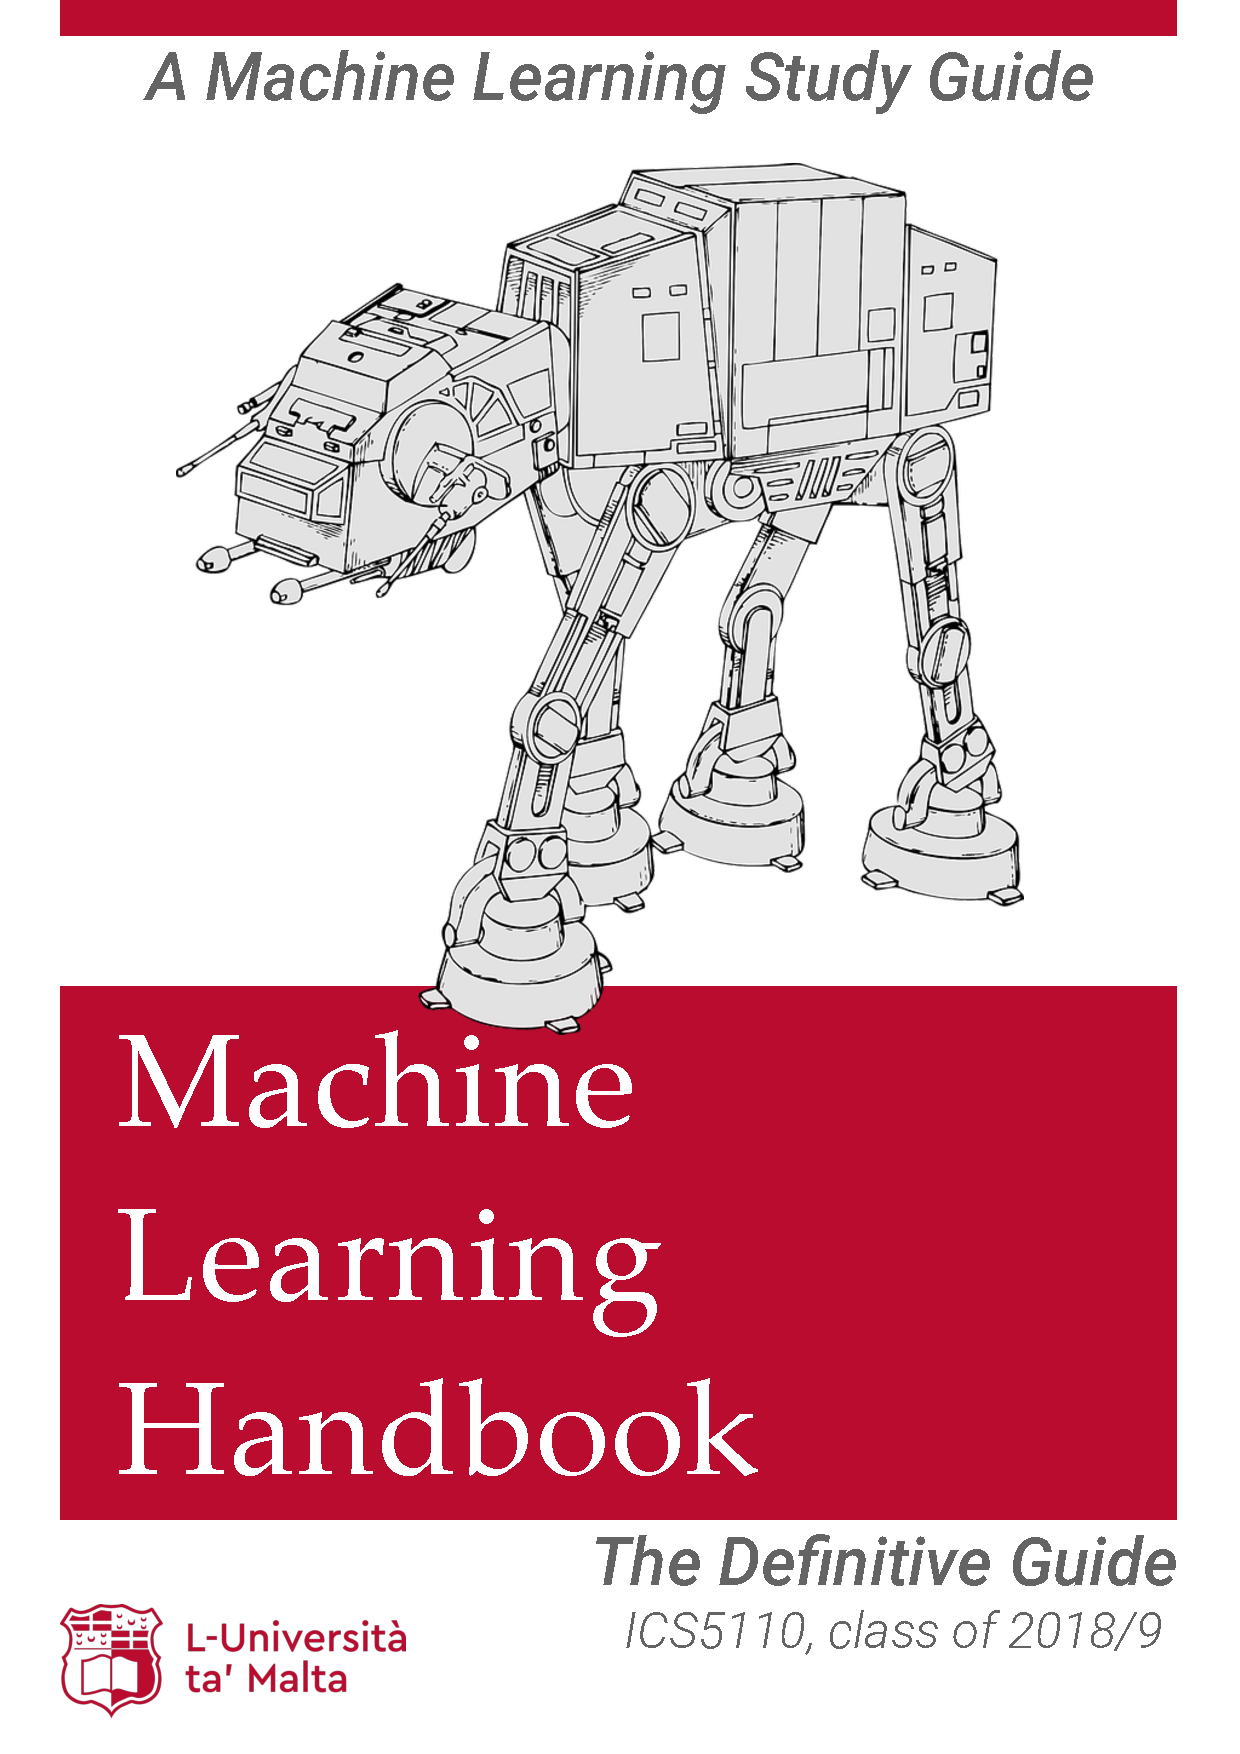
\includegraphics[width=\paperwidth]{cover/cover_oreilly_style.pdf}};
	%%\draw (current page.center) node [fill=ocre!30!white,fill opacity=0.6,text opacity=1,inner sep=1cm]{\Huge\centering\bfseries\sffamily\parbox[c][][t]{\paperwidth}{\centering The Search for a Title\\[15pt] % Book title
	%%{\Large A Profound Subtitle}\\[20pt] % Subtitle
	%%{\huge Dr. John Smith}}}; % Author name
	\end{tikzpicture}
	\vfill
	\endgroup
	

% Front matter
\frontmatter

% r.3 full title page
%% \maketitle


% v.4 copyright page
\newpage
\begin{fullwidth}
~\vfill
\thispagestyle{empty}
\setlength{\parindent}{0pt}
\setlength{\parskip}{\baselineskip}
\begin{figure*}[h]
	
\includegraphics[width=2.5in]{UMLOGO_redRGB.png}%
\end{figure*}

\par Copyright \copyright\ \the\year\ \ics\ class of 2018/9, University of Malta.

\par\smallcaps{Jean-Paul Ebejer, Dylan Seychell, Lara Marie Demajo, Keith Mintoff\hl{ADD YOUR NAME TO THIS LIST} } %TODO

\par Licensed under the Apache License, Version 2.0 (the ``License''); you may not
use this file except in compliance with the License. You may obtain a copy
of the License at \url{http://www.apache.org/licenses/LICENSE-2.0}. Unless
required by applicable law or agreed to in writing, software distributed
under the License is distributed on an \smallcaps{``AS IS'' BASIS, WITHOUT
WARRANTIES OR CONDITIONS OF ANY KIND}, either express or implied. See the
License for the specific language governing permissions and limitations
under the License.\index{license}

\par\textit{First printing, \monthyear}
\end{fullwidth}

% r.5 contents
\tableofcontents

%%\listoffigures

%%\listoftables

% r.9 introduction
\cleardoublepage
\chapter{Introduction}

This book explains popular Machine Learning terms.  We focus to explain each term comprehensively, through the use of examples and diagrams.  The description of each term is written by a student sitting in for \ics\footnote{\url{https://www.um.edu.mt/courses/studyunit/ICS5110}} at the University of Malta (class 2018/2019).  This study-unit is part of the MSc.\ in AI offered by the Department of Artificial Intelligence, Faculty of ICT.

%%
% Start the main matter (normal chapters)
\mainmatter

%% JP's example file -- file must be stored in directory "terms" and have
%% the term and initials of the student in the filename.
%% \chapter[On the Use of the tufte-book Document Class]{On the Use of the \texttt{tufte-book} Document Class}
\label{ch:tufte-book}



The \TL document classes define a style similar to the
style Edward Tufte uses in his books and handouts.  Tufte's style is known
for its extensive use of sidenotes, tight integration of graphics with
text, and well-set typography.  This document aims to be at once a
demonstration of the features of the \TL document classes
and a style guide to their use.

\section{Page Layout}\label{sec:page-layout}
\subsection{Headings}\label{sec:headings}\index{headings}
This style provides \textsc{a}- and \textsc{b}-heads (that is,
\Verb|\section| and \Verb|\subsection|), demonstrated above.

If you need more than two levels of section headings, you'll have to define
them yourself at the moment; there are no pre-defined styles for anything below
a \Verb|\subsection|.  As Bringhurst points out in \textit{The Elements of
Typographic Style},\cite{Bringhurst2005} you should ``use as many levels of
headings as you need: no more, and no fewer.''

The \TL classes will emit an error if you try to use
\linebreak\Verb|\subsubsection| and smaller headings.

% let's start a new thought -- a new section
\newthought{In his later books},\cite{Tufte2006} Tufte
starts each section with a bit of vertical space, a non-indented paragraph,
and sets the first few words of the sentence in \textsc{small caps}.  To
accomplish this using this style, use the \doccmddef{newthought} command:
\begin{docspec}
  \doccmd{newthought}\{In his later books\}, Tufte starts\ldots
\end{docspec}

\bigskip
\begin{center}
\footnotesize
\begin{tabular}{lllll}
\toprule
Feature & \vdqi & \ei & \ve & \be \\
\midrule
Author & & & & \\
\quad Typeface & serif   & serif   & serif   & sans serif \\
\quad Style    & italics & italics & italics & upright, caps \\
\quad Size     & 24 pt   & 20 pt   & 20 pt   & 20 pt \\
\addlinespace
Title & & & & \\
\quad Typeface & serif   & serif   & serif   & sans serif \\
\quad Style    & upright & italics & upright & upright, caps \\
\quad Size     & 36 pt   & 48 pt   & 48 pt   & 36 pt \\
\addlinespace
Subtitle & & & & \\
\quad Typeface & \na     & \na     & serif   & \na \\
\quad Style    & \na     & \na     & upright & \na \\
\quad Size     & \na     & \na     & 20 pt   & \na \\
\addlinespace
Edition & & & & \\
\quad Typeface & sans serif    & \na  & \na  & \na \\
\quad Style    & upright, caps & \na  & \na  & \na \\
\quad Size     & 14 pt         & \na  & \na  & \na \\
\addlinespace
Publisher & & & & \\
\quad Typeface & serif   & serif   & serif   & sans serif \\
\quad Style    & italics & italics & italics & upright, caps \\
\quad Size     & 14 pt   & 14 pt   & 14 pt   & 14 pt \\
\bottomrule
\end{tabular}
\end{center}


\section{Sidenotes}\label{sec:sidenotes}
One of the most prominent and distinctive features of this style is the
extensive use of sidenotes.  There is a wide margin to provide ample room
for sidenotes and small figures.  Any \doccmd{footnote}s will automatically
be converted to sidenotes.\footnote{This is a sidenote that was entered
using the \texttt{\textbackslash footnote} command.}  If you'd like to place ancillary
information in the margin without the sidenote mark (the superscript
number), you can use the \doccmd{marginnote} command.\marginnote{This is a
margin note.  Notice that there isn't a number preceding the note, and
there is no number in the main text where this note was written.}

The specification of the \doccmddef{sidenote} command is:
\begin{docspec}
  \doccmd{sidenote}[\docopt{number}][\docopt{offset}]\{\docarg{Sidenote text.}\}
\end{docspec}

Both the \docopt{number} and \docopt{offset} arguments are optional.  If you
provide a \docopt{number} argument, then that number will be used as the
sidenote number.  It will change of the number of the current sidenote only and
will not affect the numbering sequence of subsequent sidenotes.

Sometimes a sidenote may run over the top of other text or graphics in the
margin space.  If this happens, you can adjust the vertical position of the
sidenote by providing a dimension in the \docopt{offset} argument.  Some
examples of valid dimensions are:
\begin{docspec}
  \ttfamily 1.0in \qquad 2.54cm \qquad 254mm \qquad 6\Verb|\baselineskip|
\end{docspec}
If the dimension is positive it will push the sidenote down the page; if the
dimension is negative, it will move the sidenote up the page.

While both the \docopt{number} and \docopt{offset} arguments are optional, they
must be provided in order.  To adjust the vertical position of the sidenote
while leaving the sidenote number alone, use the following syntax:
\begin{docspec}
  \doccmd{sidenote}[][\docopt{offset}]\{\docarg{Sidenote text.}\}
\end{docspec}
The empty brackets tell the \Verb|\sidenote| command to use the default
sidenote number.

If you \emph{only} want to change the sidenote number, however, you may
completely omit the \docopt{offset} argument:
\begin{docspec}
  \doccmd{sidenote}[\docopt{number}]\{\docarg{Sidenote text.}\}
\end{docspec}

The \doccmddef{marginnote} command has a similar \docarg{offset} argument:
\begin{docspec}
  \doccmd{marginnote}[\docopt{offset}]\{\docarg{Margin note text.}\}
\end{docspec}

\section{References}
References are placed alongside their citations as sidenotes,
as well.  This can be accomplished using the normal \doccmddef{cite}
command.\sidenote{The first paragraph of this document includes a citation.}

The complete list of references may also be printed automatically by using
the \doccmddef{bibliography} command.  (See the end of this document for an
example.)  If you do not want to print a bibliography at the end of your
document, use the \doccmddef{nobibliography} command in its place.  

To enter multiple citations at one location,\cite[-3\baselineskip]{Tufte2006,Tufte1990} you can
provide a list of keys separated by commas and the same optional vertical
offset argument: \Verb|\cite{Tufte2006,Tufte1990}|.  
\begin{docspec}
  \doccmd{cite}[\docopt{offset}]\{\docarg{bibkey1,bibkey2,\ldots}\}
\end{docspec}

\section{Figures and Tables}\label{sec:figures-and-tables}
Images and graphics play an integral role in Tufte's work.
In addition to the standard \docenvdef{figure} and \docenvdef{tabular} environments,
this style provides special figure and table environments for full-width
floats.

Full page--width figures and tables may be placed in \docenvdef{figure*} or
\docenvdef{table*} environments.  To place figures or tables in the margin,
use the \docenvdef{marginfigure} or \docenvdef{margintable} environments as follows
(see figure~\ref{fig:marginfig}):

\begin{marginfigure}%
  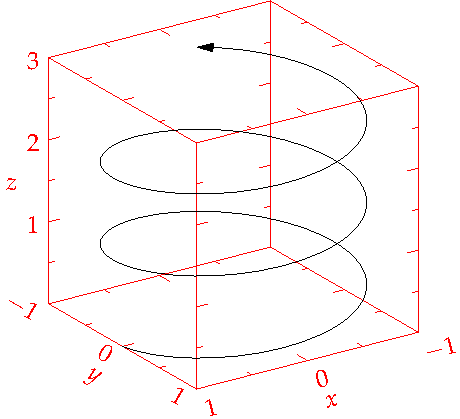
\includegraphics[width=\linewidth]{helix}
  \caption{This is a margin figure.  The helix is defined by 
    $x = \cos(2\pi z)$, $y = \sin(2\pi z)$, and $z = [0, 2.7]$.  The figure was
    drawn using Asymptote (\url{http://asymptote.sf.net/}).}
  \label{fig:marginfig}
\end{marginfigure}

\begin{docspec}
\textbackslash begin\{marginfigure\}\\
  \qquad\textbackslash includegraphics\{helix\}\\
  \qquad\textbackslash caption\{This is a margin figure.\}\\
  \qquad\textbackslash label\{fig:marginfig\}\\
\textbackslash end\{marginfigure\}\\
\end{docspec}

The \docenv{marginfigure} and \docenv{margintable} environments accept an optional parameter \docopt{offset} that adjusts the vertical position of the figure or table.  See the ``\nameref{sec:sidenotes}'' section above for examples.  The specifications are:
\begin{docspec}
  \textbackslash{begin\{marginfigure\}[\docopt{offset}]}\\
  \qquad\ldots\\
  \textbackslash{end\{marginfigure\}}\\
  \mbox{}\\
  \textbackslash{begin\{margintable\}[\docopt{offset}]}\\
  \qquad\ldots\\
  \textbackslash{end\{margintable\}}\\
\end{docspec}

Figure~\ref{fig:fullfig} is an example of the \docenv{figure*}
environment and figure~\ref{fig:textfig} is an example of the normal
\docenv{figure} environment.

\begin{figure*}[h]
  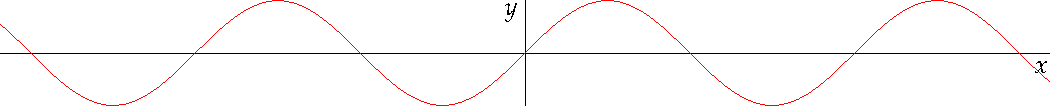
\includegraphics[width=\linewidth]{sine.pdf}%
  \caption{This graph shows $y = \sin x$ from about $x = [-10, 10]$.
  \emph{Notice that this figure takes up the full page width.}}%
  \label{fig:fullfig}%
\end{figure*}\FloatBarrier
\begin{figure}
  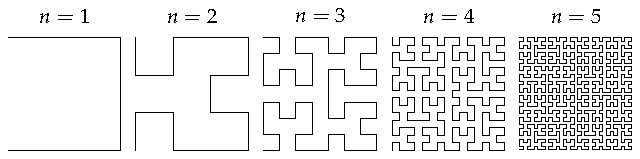
\includegraphics{hilbertcurves.pdf}
%  \checkparity This is an \pageparity\ page.%
  \caption[Hilbert curves of various degrees $n$.][6pt]{Hilbert curves of various degrees $n$. \emph{Notice that this figure only takes up the main textblock width.}}
  \label{fig:textfig}
  %\zsavepos{pos:textfig}
\end{figure}

As with sidenotes and marginnotes, a caption may sometimes require vertical
adjustment. The \doccmddef{caption} command now takes a second optional
argument that enables you to do this by providing a dimension \docopt{offset}.
You may specify the caption in any one of the following forms:
\begin{docspec}
  \doccmd{caption}\{\docarg{long caption}\}\\
  \doccmd{caption}[\docarg{short caption}]\{\docarg{long caption}\}\\
  \doccmd{caption}[][\docopt{offset}]\{\docarg{long caption}\}\\
  \doccmd{caption}[\docarg{short caption}][\docopt{offset}]%
                  \{\docarg{long caption}\}
\end{docspec}
A positive \docopt{offset} will push the caption down the page. The short
caption, if provided, is what appears in the list of figures/tables, otherwise
the ``long'' caption appears there. Note that although the arguments
\docopt{short caption} and \docopt{offset} are both optional, they must be
provided in order. Thus, to specify an \docopt{offset} without specifying a
\docopt{short caption}, you must include the first set of empty brackets
\Verb|[]|, which tell \doccmd{caption} to use the default ``long'' caption. As
an example, the caption to figure~\ref{fig:textfig} above was given in the form
\begin{docspec}
  \doccmd{caption}[Hilbert curves...][6pt]\{Hilbert curves...\}
\end{docspec}

Table~\ref{tab:normaltab} shows table created with the \docpkg{booktabs}
package.  Notice the lack of vertical rules---they serve only to clutter
the table's data.

\begin{table}[ht]
  \centering
  \fontfamily{ppl}\selectfont
  \begin{tabular}{ll}
    \toprule
    Margin & Length \\
    \midrule
    Paper width & \unit[8\nicefrac{1}{2}]{inches} \\
    Paper height & \unit[11]{inches} \\
    Textblock width & \unit[6\nicefrac{1}{2}]{inches} \\
    Textblock/sidenote gutter & \unit[\nicefrac{3}{8}]{inches} \\
    Sidenote width & \unit[2]{inches} \\
    \bottomrule
  \end{tabular}
  \caption{Here are the dimensions of the various margins used in the Tufte-handout class.}
  \label{tab:normaltab}
  %\zsavepos{pos:normaltab}
\end{table}

\newthought{Occasionally} \LaTeX{} will generate an error message:\label{err:too-many-floats}
\begin{docspec}
  Error: Too many unprocessed floats
\end{docspec}
\LaTeX{} tries to place floats in the best position on the page.  Until it's
finished composing the page, however, it won't know where those positions are.
If you have a lot of floats on a page (including sidenotes, margin notes,
figures, tables, etc.), \LaTeX{} may run out of ``slots'' to keep track of them
and will generate the above error.

\LaTeX{} initially allocates 18 slots for storing floats.  To work around this
limitation, the \TL document classes provide a \doccmddef{morefloats} command
that will reserve more slots.

The first time \doccmd{morefloats} is called, it allocates an additional 34
slots.  The second time \doccmd{morefloats} is called, it allocates another 26
slots.

The \doccmd{morefloats} command may only be used two times.  Calling it a
third time will generate an error message.  (This is because we can't safely
allocate many more floats or \LaTeX{} will run out of memory.)

If, after using the \doccmd{morefloats} command twice, you continue to get the
\texttt{Too many unprocessed floats} error, there are a couple things you can
do.

The \doccmddef{FloatBarrier} command will immediately process all the floats
before typesetting more material.  Since \doccmd{FloatBarrier} will start a new
paragraph, you should place this command at the beginning or end of a
paragraph.

The \doccmddef{clearpage} command will also process the floats before
continuing, but instead of starting a new paragraph, it will start a new page.

You can also try moving your floats around a bit: move a figure or table to the
next page or reduce the number of sidenotes.  (Each sidenote actually uses
\emph{two} slots.)

After the floats have placed, \LaTeX{} will mark those slots as unused so they
are available for the next page to be composed.

\section{Captions}
You may notice that the captions are sometimes misaligned.
Due to the way \LaTeX's float mechanism works, we can't know for sure where it
decided to put a float. Therefore, the \TL document classes provide commands to
override the caption position.

\paragraph{Vertical alignment} To override the vertical alignment, use the
\doccmd{setfloatalignment} command inside the float environment.  For
example:

\begin{fullwidth}
\begin{docspec}
  \textbackslash begin\{figure\}[btp]\\
  \qquad \textbackslash includegraphics\{sinewave\}\\
  \qquad \textbackslash caption\{This is an example of a sine wave.\}\\
  \qquad \textbackslash label\{fig:sinewave\}\\
  \qquad \hlred{\textbackslash setfloatalignment\{b\}\% forces caption to be bottom-aligned}\\
  \textbackslash end\{figure\}
\end{docspec}
\end{fullwidth}

\noindent The syntax of the \doccmddef{setfloatalignment} command is:

\begin{docspec}
  \doccmd{setfloatalignment}\{\docopt{pos}\}
\end{docspec}

\noindent where \docopt{pos} can be either \texttt{b} for bottom-aligned
captions, or \texttt{t} for top-aligned captions.

\paragraph{Horizontal alignment}\label{par:overriding-horizontal}
To override the horizontal alignment, use either the \doccmd{forceversofloat}
or the \doccmd{forcerectofloat} command inside of the float environment.  For
example:

\begin{fullwidth}
\begin{docspec}
  \textbackslash begin\{figure\}[btp]\\
  \qquad \textbackslash includegraphics\{sinewave\}\\
  \qquad \textbackslash caption\{This is an example of a sine wave.\}\\
  \qquad \textbackslash label\{fig:sinewave\}\\
  \qquad \hlred{\textbackslash forceversofloat\% forces caption to be set to the left of the float}\\
  \textbackslash end\{figure\}
\end{docspec}
\end{fullwidth}

The \doccmddef{forceversofloat} command causes the algorithm to assume the
float has been placed on a verso page---that is, a page on the left side of a
two-page spread.  Conversely, the \doccmddef{forcerectofloat} command causes
the algorithm to assume the float has been placed on a recto page---that is, a
page on the right side of a two-page spread.


\section{Full-width text blocks}

In addition to the new float types, there is a \docenvdef{fullwidth}
environment that stretches across the main text block and the sidenotes
area.

\begin{Verbatim}
\begin{fullwidth}
Lorem ipsum dolor sit amet...
\end{fullwidth}
\end{Verbatim}

\begin{fullwidth}
\small\itshape\lipsum[1]
\end{fullwidth}

\section{Typography}\label{sec:typography}

\subsection{Typefaces}\label{sec:typefaces}\index{typefaces}
If the Palatino, \textsf{Helvetica}, and \texttt{Bera Mono} typefaces are installed, this style
will use them automatically.  Otherwise, we'll fall back on the Computer Modern
typefaces.

\subsection{Letterspacing}\label{sec:letterspacing}
This document class includes two new commands and some improvements on
existing commands for letterspacing.

When setting strings of \allcaps{ALL CAPS} or \smallcaps{small caps}, the
letter\-spacing---that is, the spacing between the letters---should be
increased slightly.\cite{Bringhurst2005}  The \doccmddef{allcaps} command has proper letterspacing for
strings of \allcaps{FULL CAPITAL LETTERS}, and the \doccmddef{smallcaps} command
has letterspacing for \smallcaps{small capital letters}.  These commands
will also automatically convert the case of the text to upper- or
lowercase, respectively.

The \doccmddef{textsc} command has also been redefined to include
letterspacing.  The case of the \doccmd{textsc} argument is left as is,
however.  This allows one to use both uppercase and lowercase letters:
\textsc{The Initial Letters Of The Words In This Sentence Are Capitalized.}



\section{Document Class Options}\label{sec:options}

\index{class options|(}
The \doccls{tufte-book} class is based on the \LaTeX\ \doccls{book}
document class.  Therefore, you can pass any of the typical book
options.  There are a few options that are specific to the
\doccls{tufte-book} document class, however.

The \docclsoptdef{a4paper} option will set the paper size to \smallcaps{A4} instead of
the default \smallcaps{US} letter size.

The \docclsoptdef{sfsidenotes} option will set the sidenotes and title block in a 
\textsf{sans serif} typeface instead of the default roman.

The \docclsoptdef{twoside} option will modify the running heads so that the page
number is printed on the outside edge (as opposed to always printing the page
number on the right-side edge in \docclsoptdef{oneside} mode).  

The \docclsoptdef{symmetric} option typesets the sidenotes on the outside edge of
the page.  This is how books are traditionally printed, but is contrary to
Tufte's book design which sets the sidenotes on the right side of the page.
This option implicitly sets the \docclsopt{twoside} option.

The \docclsoptdef{justified} option sets all the text fully justified (flush left
and right).  The default is to set the text ragged right.  
The body text of Tufte's books are set ragged right.  This prevents
needless hyphenation and makes it easier to read the text in the slightly
narrower column.

The \docclsoptdef{bidi} option loads the \docpkg{bidi} package which is used with
\tXeLaTeX\ to typeset bi-directional text.  Since the \docpkg{bidi}
package needs to be loaded before the sidenotes and cite commands are defined,
it can't be loaded in the document preamble.

The \docclsoptdef{debug} option causes the \TL classes to output debug
information to the log file which is useful in troubleshooting bugs.  It will
also cause the graphics to be replaced by outlines.

The \docclsoptdef{nofonts} option prevents the \TL classes from
automatically loading the Palatino and Helvetica typefaces.  You should use
this option if you wish to load your own fonts.  If you're using \tXeLaTeX, this
option is implied (\ie, the Palatino and Helvetica fonts aren't loaded if you
use \tXeLaTeX).  

The \docclsoptdef{nols} option inhibits the letterspacing code.  The \TL\
classes try to load the appropriate letterspacing package (either pdf\TeX's
\docpkg{letterspace} package or the \docpkg{soul} package).  If you're using
\tXeLaTeX\ with \docpkg{fontenc}, however, you should configure your own
letterspacing.  

The \docclsoptdef{notitlepage} option causes \doccmd{maketitle} to generate a title
block instead of a title page.  The \doccls{book} class defaults to a title
page and the \doccls{handout} class defaults to the title block.  There is an
analogous \docclsoptdef{titlepage} option that forces \doccmd{maketitle} to
generate a full title page instead of the title block.

The \docclsoptdef{notoc} option suppresses \TL's custom table of contents
(\textsc{toc}) design.  The current \textsc{toc} design only shows unnumbered
chapter titles; it doesn't show sections or subsections.  The \docclsopt{notoc}
option will revert to \LaTeX's \textsc{toc} design.

The \docclsoptdef{nohyper} option prevents the \docpkg{hyperref} package from
being loaded.  The default is to load the \docpkg{hyperref} package and use the
\doccmd{title} and \doccmd{author} contents as metadata for the generated
\textsc{pdf}.

\index{class options|)}


\chapter{\textit{}Cross-Validation}
\label{ch:cross-validation}\index{cross-validation}

Cross-validation (CV) is an estimation method used on supervised learning algorithms to assess their ability to predict the output of unseen data \cite[-3\baselineskip]{varma2006bias,kohavi1995study}. Supervised learning algorithms are computational tasks like classification or regression, that learn an input-output function based on a set of samples. Such samples are also known as the labeled training data where each example consists of an input vector and its correct output value. After the training phase, a supervised learning algorithm should be able to use the inferred function in order to map new input unseen instances, known as testing data, to their correct output values \cite{caruana2006empirical}. When the algorithm incorporates supervised feature selection, cross-validation should always be done external to the selection (feature-selection performed within every CV iteration) so as to ensure the test data remains unseen, reducing bias \cite[-3\baselineskip]{ambroise2002selection, friedman2001elements}.  Therefore, cross-validation, also known as out-of-sample testing, tests the function's ability to generalize to unseen situations \cite[-3\baselineskip]{varma2006bias,kohavi1995study}. 

Cross-validation has two types of approaches, being i) the exhaustive cross validation approach which divides all the original samples in every possible way, forming training and test sets to train and test the model, and ii) the non-exhaustive cross validation approach which does not consider all the possible ways of splitting the original samples \cite{arlot2010survey}. Each of these approaches are further divided into different cross-validation methods, which are explained below.
\\\\
\noindent\textbf{Exhaustive cross-validation}
\begin{itemize}
\item Leave-$p$-out (L$p$O) \newline \index{leave-p-out}
This method takes $p$ samples from the data set as the test set and keeps the remaining as the training set, as shown in Fig.~\ref{fig:leavep}a. This is repeated for every combination of test and training set formed from the original data set and the average error is obtained. Therefore, this method trains and tests the algorithm $n\choose p$ times when the number of samples in the original data set is $n$, becoming inapplicable when $p>1$ \cite{arlot2010survey}.

\item Leave-one-out (LOO)\newline \index{leave-one-out}
This method is a specific case of the LpO method having $p=1$. It requires less computation efforts than LpO since the process is only repeated $n choose 1$ $= n$ times, however might still be inapplicable for large values of $n$ \cite{arlot2010survey}. 
\end{itemize}

\begin{figure*}
\centering
\begin{subfigure}
  \centering
  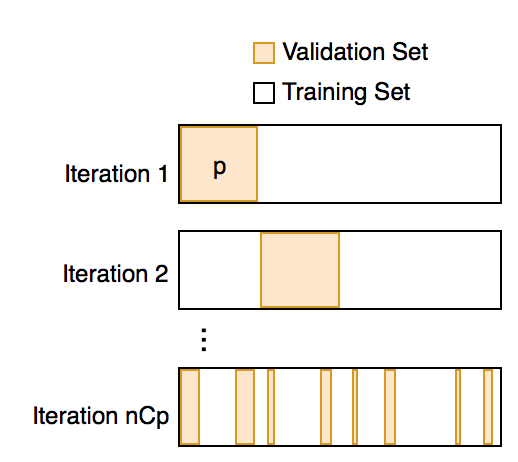
\includegraphics[width=.4\linewidth]{leavep.png}
  \caption{Leave-p-Out}
  \end{subfigure}
 \begin{subfigure}
  \centering
  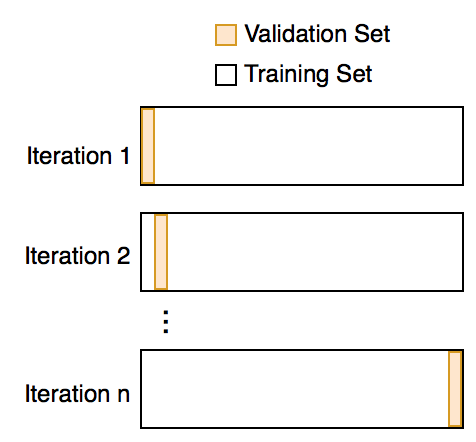
\includegraphics[width=.37\linewidth]{leave1.png}
  \caption{Leave-One-Out}
  \end{subfigure}
  \caption{Exhaustive cross-validation methods: Leave-p-Out (left) \& Leave-One-Out (right)}
  \label{fig:leavep}
\end{figure*}

\break\noindent\textbf{Non-exhaustive cross-validation}
\begin{itemize}
\item Holdout method \newline \index{holdout}
This method randomly splits the original data set into two sets being the training set and the test set. Usually, the test set is smaller than the training set so that the algorithm has more data to train on. This method involves a single run and so must be used carefully to avoid misleading results. It is therefore sometimes not considered a CV method \cite{kohavi1995study}.

\item $k$-fold\newline \index{k-fold}
This method randomly splits the original data set into $k$ equally sized subsets, as shown in Fig.~\ref{fig:kfold}. The function is then trained and validated $k$ times, each time taking a different subset as the test data and the remaining $(k-1)$ subsets as the training data, using each of the $k$ subsets as the test set once. The $k$ results are averaged to produce a single estimation. Stratified $k$-fold cross validation is a refinement of the $k$-fold method, which splits the original samples into equally sized and distributed subsets, having the same proportions of the different target labels \cite{kohavi1995study}.

\begin{figure}
\centering
  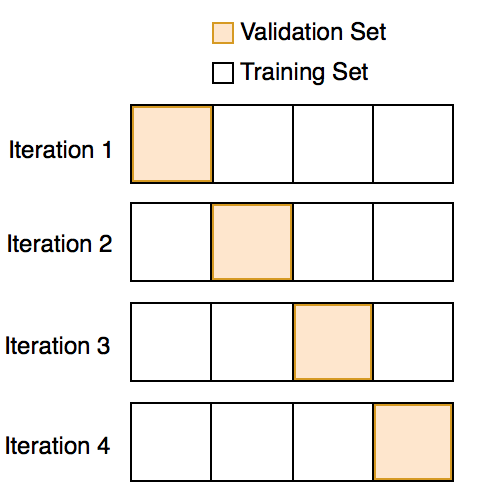
\includegraphics[width=0.5\linewidth]{kfold.png}
  \caption{$k$-Fold Cross Validation where $k$=4}
  \label{fig:kfold}
\end{figure}

\item Repeated random sub-sampling\newline \index{repeated random sub-sampling}
This method is also known as the Monte Carlo CV. It splits the data set randomly with replacement into training and test subsets using some predefined split percentage, for every run. Therefore, this generates new training and test data for each run but the test data of the different runs might contain repeated samples, unlike that of $k$-fold \cite{xu2001monte}.
\end{itemize}

All of the above cross-validation methods are used to check whether the model has been overfitted or underfitted and hence estimating the model's ability of fitting to independent data . Such ability is measured using quantitative metrics appropriate for the model and data \cite[-3\baselineskip]{kohavi1995study, arlot2010survey}. In the case of classification problems, the misclassification error rate is usually used whilst for regression problems, the mean squared error (MSE) is usually used. MSE is represented by Eq.~\ref{mse}, where n is the total number of test samples, $Y_i$ is the true value of the $i^{th}$ instance and $\hat{Y}_i$ is the predicted value of the $i^{th}$ instance.

\begin{equation}\label{mse}
MSE = \frac{1}{n}\sum^{n}_{i=1}(Y_i - \hat{Y}_i)^2
\end{equation}

Underfitting \index{underfitting} is when the model has a low degree (e.g. $y = x$, where the degree is 1) and so is not flexible enough to fit the data making the model have a low variance and high bias \cite{baumann2003cross}, as seen in Fig.~\ref{fig:models}a. Variance is the model's dependence on the training data and bias is model's assumption about the shape of the data \cite{arlot2010survey}. On the other hand, as seen in Fig.~\ref{fig:models}b, overfitting \index{overfitting} is when the model has a too high degree (e.g. $y = x^{30}$, where the degree is 30) causing it to exactly fit the data as well as the noise and so lacks the ability to generalize \cite{baumann2003cross}, making the model have a high variance. Cross-validation helps reduce this bias and variance since it uses most of the data for both fitting and testing and so helps the model learn the actual relationship within the data. This makes cross-validation a good technique for models to acquire a good bias-variance tradeoff \cite{arlot2010survey}.

\begin{figure*}
\centering
\begin{subfigure}
  \centering
  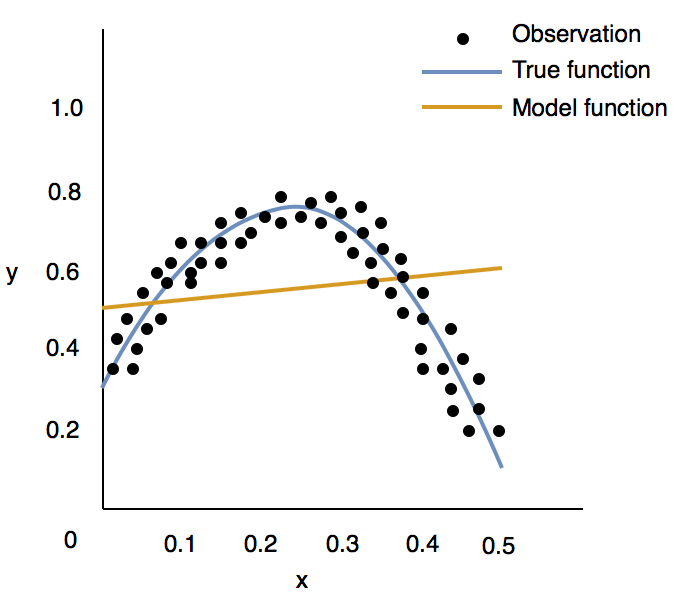
\includegraphics[width=0.4\linewidth]{underfitting.png}
  \caption{Underfitting}
  \label{fig:underfitting}
\end{subfigure}
\begin{subfigure}
  \centering
  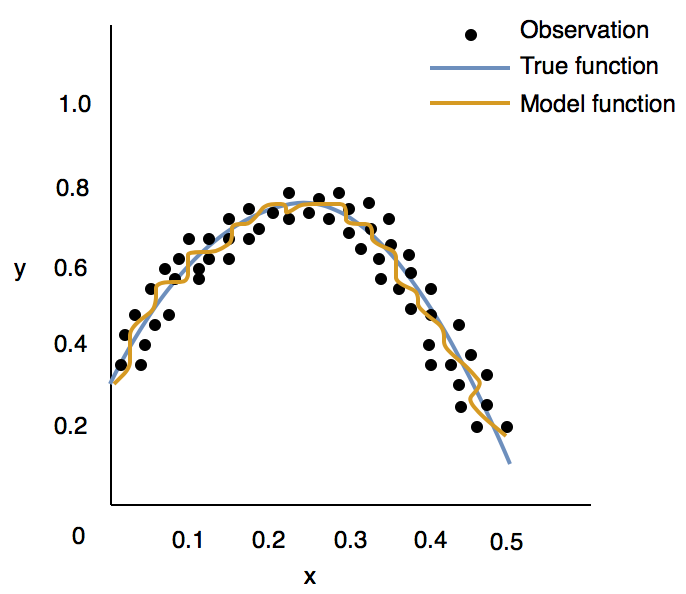
\includegraphics[width=.4\linewidth]{overfitting.png}
  \caption{Overfitting}
  \label{fig:overfitting}
\end{subfigure}
\caption{Underfitting (left) \& Overfitting (right)}
\label{fig:models}
\end{figure*}

As stated in \cite{kohavi1995study}, the LOO method gives a 0\% accuracy on the test set when the number of target labels are equal to the number of instances in the dataset. It is shown that the $k$-fold CV method gives much better results, due to its lower variance, especially when $k = {10, 20}$. Furthermore, R. Kohavi et al. state that the best accuracy is achieved when using the stratified cross-validation method, since this has the least bias.

Therefore, lets take an example using the stratified $k$-fold cross-validation method with $k=10$. Let's say that we are trying to solve age group classification, using eight non-overlapping age groups being 0-5, 6-10, 11-20, 21-30, 31-40, 41-50, 51-60, and 61+. We are using the FG-NET labelled data set, which contains around 1000 images of individuals aged between 0 and 69. Before we can start training our model (e.g. CNN), we must divide our data set into training and test subsets and this is where cross validation comes in. Therefore, we start by taking the 1000 images of our data set and splitting them according to their target class. Let us assume we have an equal amount of 125 $(1000/8)$ images per class\footnote{Down-sampling or up-sampling are common techniques used when there is an unequal amount of samples for the different classes.}. As depicted in Fig.~\ref{fig:example}, we can now start forming our 10 folds by taking 10\% of each age-group bucket, randomly without replacement. Hence, we will end up with 10 subsets of 100 images that are equally distributed along all age-groups. With these subsets, we can estimate our model's accuracy with a lower bias-variance tradeoff. Since we are using 10-fold CV, we will train and test our model 10 times. For the first iteration, we shall use subset 1 as the validation set and subsets 2 to 10 as the training set, for the second iteration we use subset 2 as the test set and subsets 1 plus 3 to 10 as our training set, and so on (as shown in Fig.~\ref{fig:kfold}). For each iteration we use the misclassification error rate to obtain an accuracy value and we finally average the 10 accuracy rates to obtain the global accuracy of our model when solving age group classification, given the FG-NET data set. Hence, we have now estimated the prediction error of the model and have an idea of how well our model performs in solving such a problem. It is important to note that cross-validation is \textit{just} an estimation method and when using our model in real-life applications we do not apply CV but rather train our model with all the data we have.

\begin{figure*}
\centering
  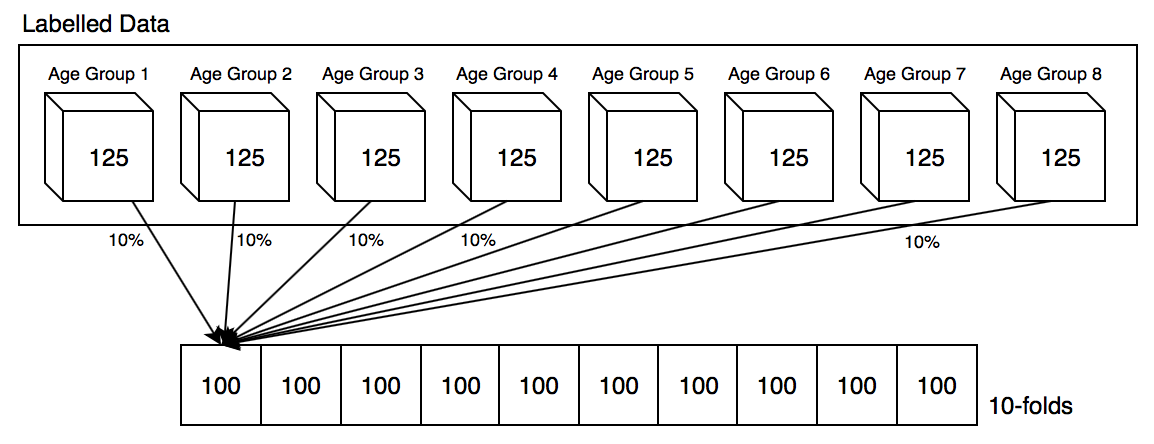
\includegraphics[width=0.88\linewidth]{example-cv.png}
  \caption{Stratified 10-fold cross-validation on 1000 labelled images of 8 different classes}
  \label{fig:example}
\end{figure*}

As concluded by \cite{varma2006bias}, cross-validation is well implemented when everything is taken place within every CV iteration (including preprocessing, feature-selection, learning new algorithm parameter values, etc.), and the least bias can be achieved when using nested CV methods.



\index{class options|)}
\chapter[Activation Functions]{Activation Functions}
\label{ch:activation-functions}\index{activation functions|(}
``Neural networks were originally conceived as a model that would imitate the function of the human brain---a set of neurons joined together by a set of connections. Neurons, in this context, are composed of a weighted sum of their inputs followed by a nonlinear function, which is also known as an activation function.'' \citep{caterini2018}

Activation Functions are used in Artificial Neural Networks to determine whether the output of the neuron should be considered further or ignored. If the activation function chooses to continue considering the output of a neuron, we say that the neuron has been activated. The output of the activation function is what is passed on to the subsequent layer in a multilayer neural network. To determine whether a neuron should be activated, the activation function takes the output of a neuron and transforms it into a value commonly bound to a specific range, typically from $0$ to $1$ or $-1$ to $1$ depending on the which activation function is applied.

\section{Step Function}\label{sec:step-function}\index{step function}

\begin{marginfigure}
  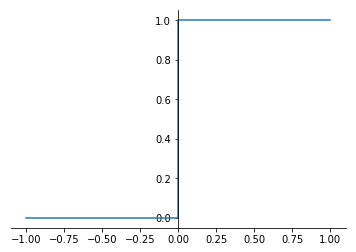
\includegraphics{graphics/activation_functions/step_function.png}
  \label{fig:stepfunction}
  \caption{
    A graph of the step function. 
  }
\end{marginfigure}

\begin{equation}\label{stepfunction}
    f(x) =
    \begin{dcases*}
        0 & \text{for \(x < 0\)} \\
        1 & \text{for \(x \geq 0\)} \\
    \end{dcases*}
\end{equation}

\begin{equation}\label{stepfunctionderivative}
    \frac{d}{d(x)}f(x) =
      \begin{dcases*}
                                       0 & \text{for \(x \neq 0\)} \\
                                       ? & \text{for \(x = 0\)} \\
      \end{dcases*}
\end{equation}

The Heavside step function, represented by Eq.~\ref{stepfunction}, is one of the simplest activation functions that can be used in a neural network. This activation function returns $0$ if the input of a node is less than a predetermined threshold (typically $0$), or otherwise it returns $1$ if the output of the node is greater than or equal to the threshold. This function was first used in a machine learning context in 1957 by Frank Rosenblatt in his seminal work describing the perceptron, the precursor to the modern day neural network \citep{rosenblatt1957perceptron}. 

Nowadays, the step function is seldom used in practice as it cannot be used to classify more than one class. Furthermore, since the derivative of this function, represented by Eq.~\ref{stepfunctionderivative}, is $0$, gradient descent algorithms are not be able to progressively update the weights of a network that makes use of this function \citep{Snyman2005}.

\section{Linear Functions}\label{sec:linear-function}\index{linear activation function}

A linear activation function seeks to solve some of the shortcomings of the step function. The output produced by a linear activation function is proportional to the input. While a linear activation function could be used for multi-class problems, it can on be used on problems that are linearly separable. Linear functions can also run into problems with gradient descent algorithms, as the derivative of a linear function is a constant. Additionally, since the output of the linear function is not bound to any range, it could be susceptible to a common problem when training deep neural networks called the exploding gradient problem, which can make learning unstable \citep{goodfellow2016deeplearning}.

\section{Sigmoid Function}\label{sec:sigmoid}\index{sigmoid function}

\begin{marginfigure}
  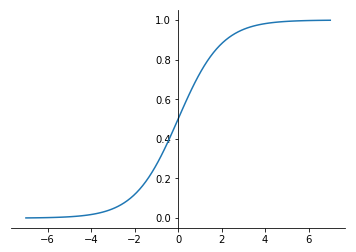
\includegraphics{graphics/activation_functions/sigmoid_function.png}
  \label{fig:sigmoidfunction}
  \caption{
    A graph of the sigmoid function.
  }
\end{marginfigure}

\begin{equation}\label{sigmoidfunction}
    f(x) = \frac{1}{(1 + e^{-x})}
\end{equation}

\begin{equation}\label{sigmoidfunctionderivative}
    \frac{d}{d(x)}f(x) = f(x)(1-f(x))
\end{equation}

The sigmoid function or logistic function, represented by  Eq.~\ref{sigmoidfunction}, is one of the most commonly used activation functions in neural networks, because of its simplicity and desirable properties. The use of this function in neural networks was first introduced by Rummelhart, Hinton and Williams in one of the most important papers in the field of machine learning, which described the back-propagation algorithm and the introduction of hidden layers, giving rise to modern day neural networks \citep{DavidE.Rumelhart1986Lrbb}.  The values produced by the step function are bound between $0$ and $1$, both not inclusive, which help manage the exploding gradient problem. The derivative of this function (Eq.~\ref{sigmoidfunctionderivative})  produces a very steep gradient for a relatively small range of values, typically in the range of $-2$ to $2$. This means that for most inputs that the function receives it will return values that are very close to either $0$ or $1$.

On the other hand, this last property makes the sigmoid function very susceptible to the vanishing gradient problem \citep{bengio94}. When observing the shape of the sigmoid function we see that towards the ends of the curve, function becomes very unresponsive to changes in the input. In other words, the gradient of the function for large inputs becomes very close to $0$. 

\section{Hyperbolic Tangent}\label{sec:tanh}\index{hyperbolic tangent}
\begin{marginfigure}
  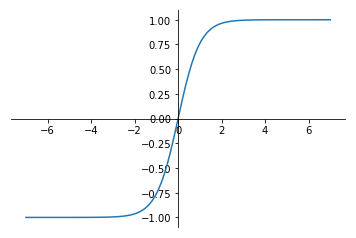
\includegraphics{graphics/activation_functions/tanh_function.png}
  \label{fig:tanhfunction}
  \caption{
    A graph of the hyperbolic tangent ($tanh$) function.
  }
\end{marginfigure}

\begin{equation}\label{tanhfunction}
    f(x) = \frac{(e^{x} - e^{-x})}{(e^{x} + e^{-x})}
\end{equation}

\begin{equation}\label{tanhfunctionderivative}
    \frac{d}{d(x)}f(x) = 1-f(x)^2.
\end{equation}

The hyperbolic tangent ($tanh$) function, represented by  Eq.~\ref{tanhfunction}, is another activation function that is sometimes used instead of sigmoid. The $tanh$ function has the same characteristics of the sigmoid function mentioned above. In fact the $tanh$ function is plotted, one can observe that it is simply a scaled version of the sigmoid function. As a result of this scaling, the tanh function has a steeper gradient in towards the origin, and it returns values between $-1$ and $1$. The derivative of the hyperbolic tangent function is represented by Eq.~\ref{tanhfunctionderivative}.

Nowadays with the rise of deep learning, these functions are becoming less commonly used. Xavier Glorot and Yoshua Bengio studied in detail the effects of the sigmoid and tanh activation functions. They note how the sigmoid function in particular is not well suited for deep networks with random initialization \citep{glorot2010understanding}.

\section{Rectified Linear Unit}\label{sec:relu}\index{rectified linear unit (relu)}
\begin{marginfigure}
  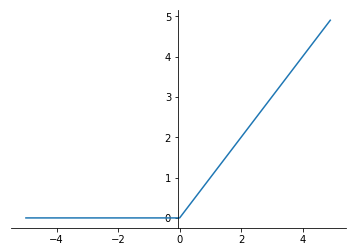
\includegraphics{graphics/activation_functions/relu_function.png}
  \label{fig:relufunction}
  \caption{
    A graph of the ReLU function.
  }
\end{marginfigure}

\begin{equation}\label{relufunction}
    f(x) =
      \begin{dcases*}
                                       0 & \text{for $x < 0$} \\
                                       x & \text{for $x \geq 0$} \\
      \end{dcases*}
\end{equation}

\begin{equation}\label{relufunctionderivative}
    \frac{d}{d(x)}f(x) =
      \begin{dcases*}
                                       0 & \text{for $x < 0$} \\
                                       1 & \text{for $x \geq 0$} \\
      \end{dcases*}
\end{equation}

The ReLU function, represented by  Eq.~\ref{relufunction}, returns $0$ if the input of the function is negative, otherwise it outputs the value of the input itself. This function is non-linear in nature even though at first glance it may seem similar to an identity function. The ReLU function is becoming one of the more commonly used activation function due to its simplicity performance, and suitability to networks with many layers. Another benefit of the ReLU function is that it produces sparse activations (not all nodes in the network are activated) unlike the sigmoid or hyperbolic tangent functions. 

The ReLU function has been used in many neural network models to improve their performance. Naid and Hinton use ReLU to improve the performance of Restricted Boltzmann Machines in object recognition \citep{Nair2010}. In 2012, a breakthrough Convolutional Neural Network (CNN) architecture called AlexNet pioneered the use of the ReLU activation function together with dropout layers to minimise over fitting in CNNs.  \citep{KrizhevskyAlex2017Icwd}. 

Unfortunately, because the gradient of the function for inputs that are negative is $0$ (Eq.~\ref{relufunctionderivative}), the ReLU function can still be susceptible to the vanishing gradient problem. To manage this problem a variant of the ReLU function, called Leaky ReLU is sometimes used. Rather than simply returning 0 for negative inputs, the leaky ReLU return a very small value such as $0.01x$. However, researchers at the University of Stanford compared the performance of Sigmoid, ReLU and Leaky ReLU functions and found that while the the performance of both the ReLU and Leaky Relu functions was better than the performance achieved with the sigmoid function, the performance of the two ReLU functions was nearly identical  \citep{maas2013rectifier}.
\index{activation functions|)}
 %TODO


%%
% The back matter contains appendices, bibliographies, indices, glossaries, etc.

\backmatter

%% \bibliography{terms/myterm_jpe} 
\bibliography{terms/crossvalidation_lmd,terms/activationfunctions_km}
\bibliographystyle{plainnat}

\printindex

\end{document}

